\documentclass[11pt]{article}
\usepackage[margin=1in]{geometry}
\usepackage{amsmath,amssymb,amsthm}
\usepackage{graphicx}
\usepackage{caption}
\usepackage{hyperref}
\usepackage{booktabs}
\usepackage{xcolor}
\usepackage{float}

\graphicspath{{figs/}}
\hypersetup{colorlinks=true, linkcolor=blue, citecolor=blue, urlcolor=blue}

\title{Chebyshev Interpolation in $\sigma{-}\delta$ Coordinates\\
\large with $S_3 \times Z_2$ Symmetry for the K=3 CRRA REE}
\author{Design note for MIZN}
\date{}

\begin{document}
\maketitle
\tableofcontents

\section{The coordinate puzzle: three agents, three perspectives}

The K=3 REE problem fixes a price function $P(u_1, u_2, u_3) \in [0,1]$ on
a 3-D cube of private signals (Fig.~\ref{fig:cube}). The fixed-point operator
$\Phi$ updates $P$ by, at each cube cell, running each agent's
Bayesian-update + clearing routine. The crucial structural fact is that
\textbf{each agent integrates over a different 2-D slice}:
\begin{itemize}
\item Agent 1 holds $u_1$ fixed, integrates over $(u_2, u_3)$.
\item Agent 2 holds $u_2$ fixed, integrates over $(u_1, u_3)$.
\item Agent 3 holds $u_3$ fixed, integrates over $(u_1, u_2)$.
\end{itemize}

\begin{figure}[H]
\centering
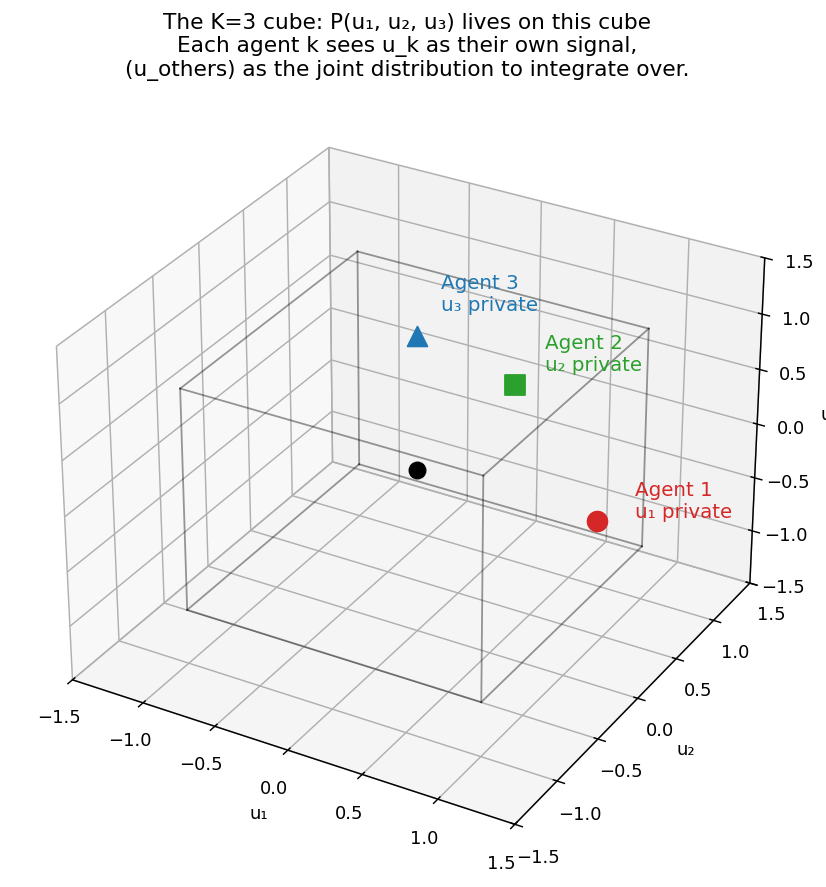
\includegraphics[width=0.7\linewidth]{01_cube.png}
\caption{The K=3 cube. Each agent's "own" axis is the one they see directly;
the orthogonal plane is what they integrate over for the Bayesian update.}
\label{fig:cube}
\end{figure}

The $\sigma$-$\delta$ rotation (which we used in the previous session's
\texttt{v11\_strict\_h0\_hardwired.py} operator) re-parametrizes each
agent's integration plane as $\Sigma = u_a + u_b$ (symmetric direction) and
$\delta = u_a - u_b$ (antisymmetric direction). This is a per-agent rotation
of the "other two" axes (Fig.~\ref{fig:perg}).

\begin{figure}[H]
\centering
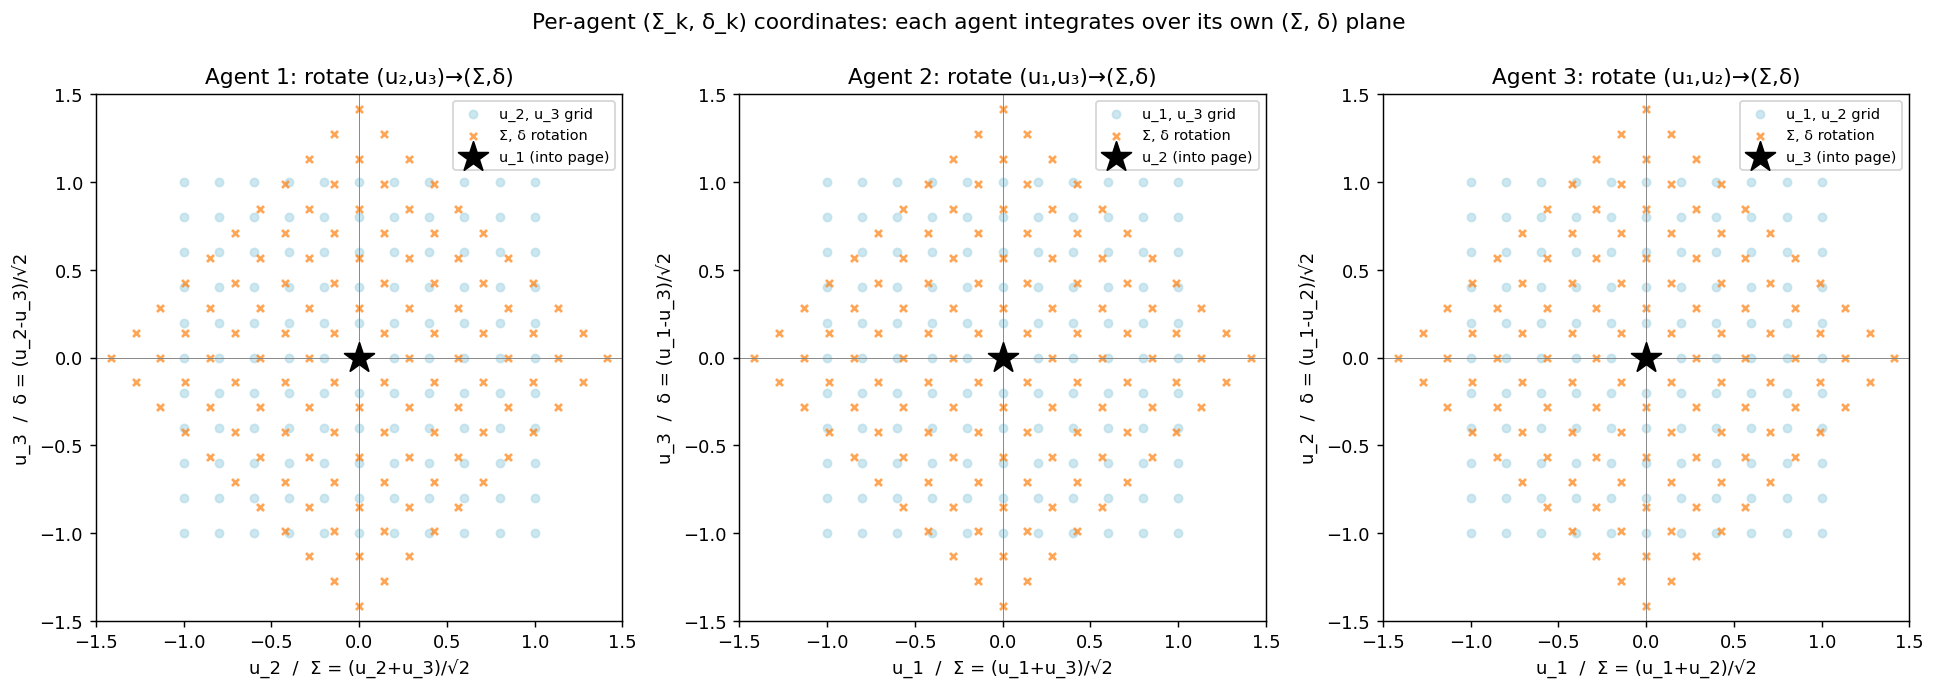
\includegraphics[width=\linewidth]{02_per_agent_rotation.png}
\caption{Per-agent $\sigma$-$\delta$ rotation. Each panel shows one agent's
orthogonal plane; the agent's own axis is into the page (black star). Blue
dots = original $(u_a, u_b)$ uniform grid. Orange crosses = rotated
$(\Sigma, \delta)$ frame. \textbf{The rotation is different for each agent} —
agent 1's $\Sigma$ is $u_2+u_3$, agent 2's $\Sigma$ is $u_1+u_3$, etc.}
\label{fig:perg}
\end{figure}

\paragraph{The puzzle.} If we want to discretize $P$ with a Chebyshev tensor
basis, we must pick \emph{one} coordinate system to store it in. Which one,
when each agent needs a different one for their slice integration?

This is the question this note addresses. The answer is: \textbf{store $P$
in canonical $(u_1,\Sigma_{23},\delta_{23})$ coordinates and use $S_3$
symmetry to evaluate it at permuted points for agents 2 and 3.} The
symmetry isn't a "nice-to-have" — it's what makes the per-agent evaluation
free instead of requiring per-agent re-interpolation.

\section{The $\sigma$-$\delta$ $\xi$-cube and Chebyshev}

We map the unbounded $u$ axes to bounded $\xi \in [-1,1]$ axes via
$\xi = \tanh(u/T)$ (or any equivalent atanh stretch). The resulting box
$\xi \in [-1,1]^3$ is the natural domain for Chebyshev (Fig.~\ref{fig:sdcube}).

\begin{figure}[H]
\centering
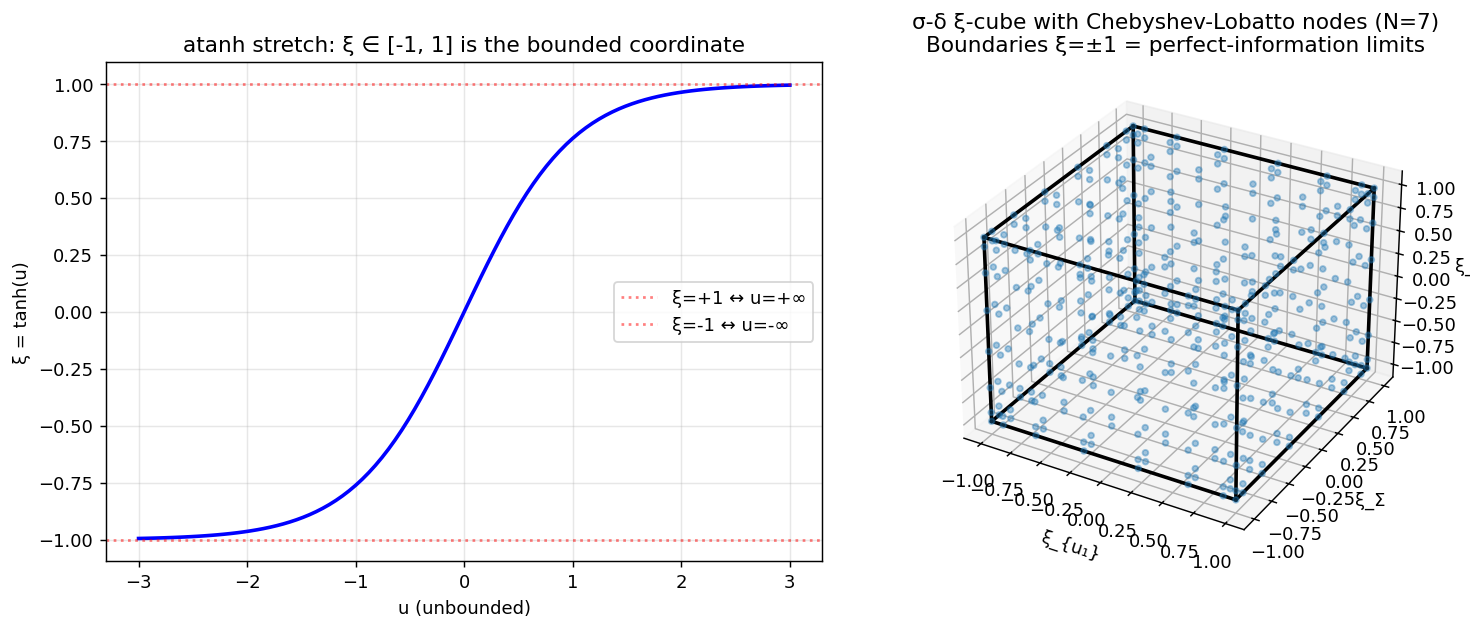
\includegraphics[width=\linewidth]{03_sigma_delta_cube.png}
\caption{Left: the $\tanh$ stretch turns the unbounded $u$ axis into the
bounded $\xi$ axis; boundaries $\xi=\pm 1$ correspond exactly to the
perfect-information limits $u=\pm\infty$ where $P=0$ or $1$ exactly. Right:
the $\sigma$-$\delta$ $\xi$-cube with Chebyshev-Lobatto nodes ($N=7$). Nodes
cluster near the boundaries — this is what prevents Runge instability.}
\label{fig:sdcube}
\end{figure}

\subsection{Chebyshev polynomial basis (primer)}

Chebyshev polynomials of the first kind, $T_n(\xi) = \cos(n\arccos\xi)$,
are the unique orthogonal polynomials on $[-1,1]$ with weight
$(1-\xi^2)^{-1/2}$. They have two properties that matter for us
(Fig.~\ref{fig:cheb}):

\begin{itemize}
\item \textbf{Spectral convergence}: for any function analytic on a
neighborhood of $[-1,1]$, the Chebyshev coefficients decay
\emph{exponentially}, $a_n \sim e^{-\alpha n}$, with $\alpha$ controlled by
how far the singularities are from $[-1,1]$.

\item \textbf{Parity property}: $T_n(-\xi) = (-1)^n T_n(\xi)$. Even-degree
$T_n$ are even; odd-degree are odd. \textbf{This is the algebraic mechanism
that makes the $Z_2$ symmetry kill half the coefficients} (Sec.~\ref{sec:Z2}).
\end{itemize}

\begin{figure}[H]
\centering
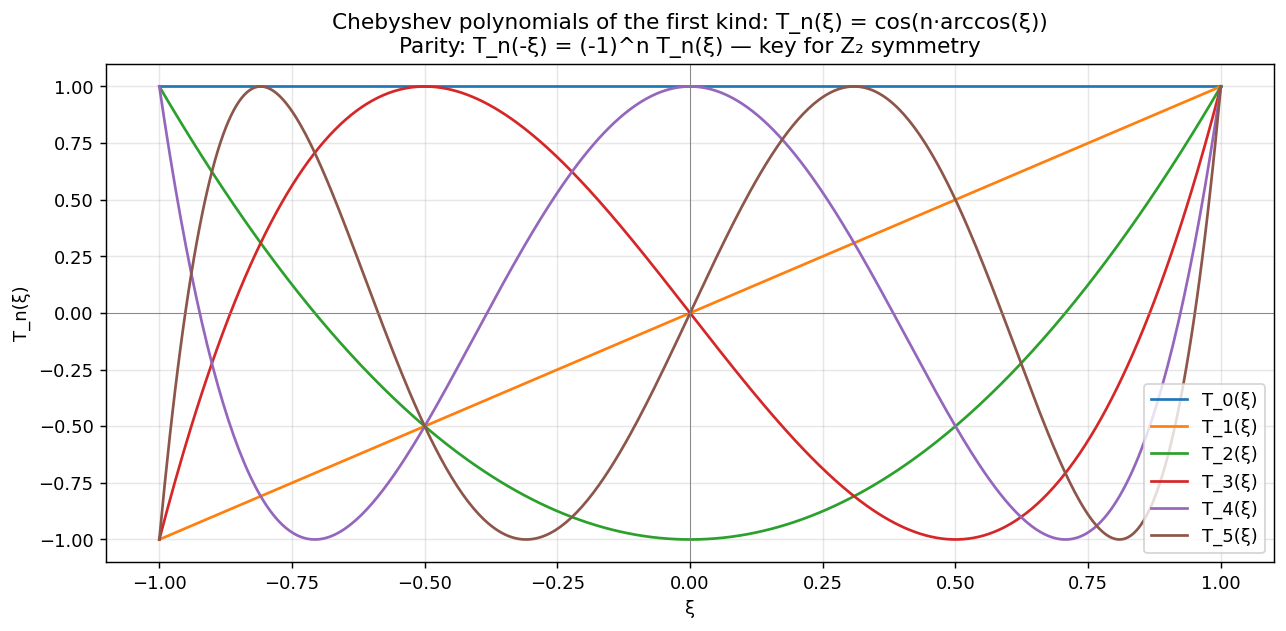
\includegraphics[width=\linewidth]{04_chebyshev_basis.png}
\caption{The first six Chebyshev polynomials $T_0, T_1, \ldots, T_5$ on
$[-1,1]$. Note the parity: $T_n(-\xi) = (-1)^n T_n(\xi)$.}
\label{fig:cheb}
\end{figure}

\subsection{Why Chebyshev-Lobatto nodes}

We collocate (sample) at the Chebyshev-Lobatto points $\xi_j = -\cos(\pi
j/N)$, $j=0,\ldots,N$. These cluster near $\xi=\pm 1$
(Fig.~\ref{fig:lobatto}), which is what prevents the Runge instability that
afflicts polynomial fits at uniform nodes.

\begin{figure}[H]
\centering
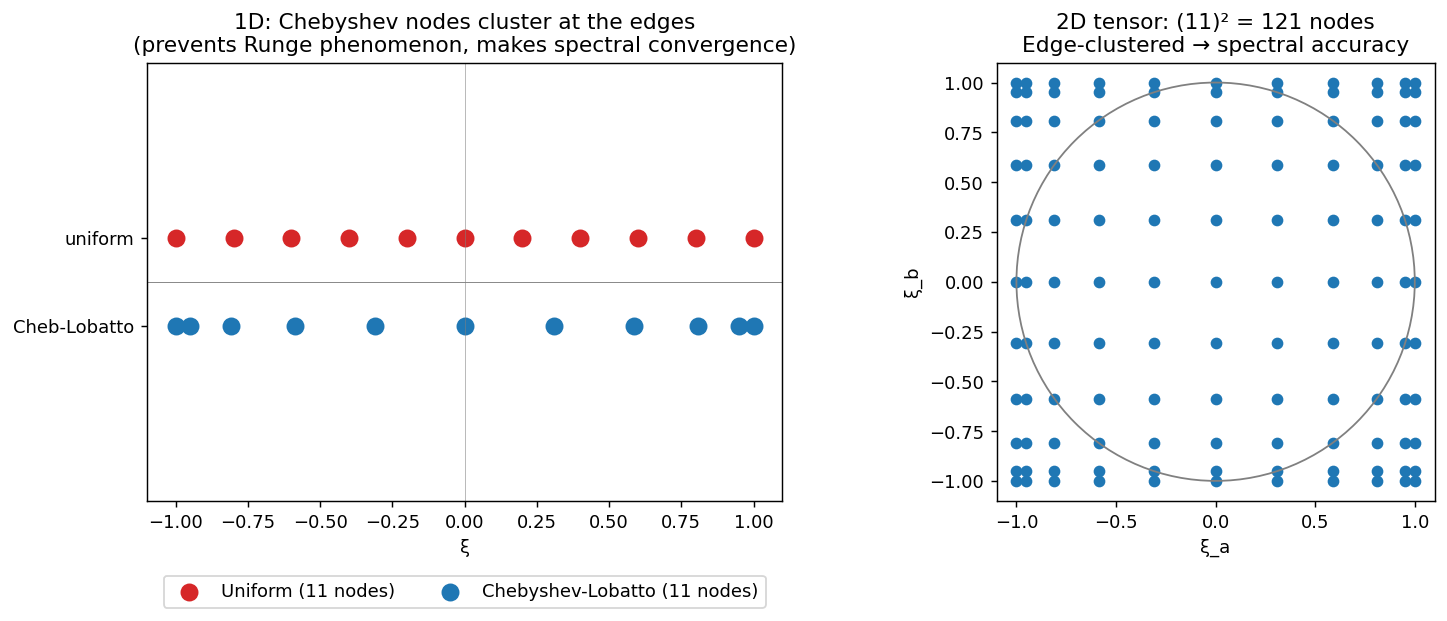
\includegraphics[width=\linewidth]{05_lobatto_nodes.png}
\caption{Left: uniform nodes (red) vs Chebyshev-Lobatto nodes (blue) in 1D.
The Lobatto nodes cluster at the boundaries — exactly where polynomial
fits go wrong with uniform sampling. Right: 2D tensor of Lobatto nodes
($(N+1)^2$ points).}
\label{fig:lobatto}
\end{figure}

The empirical payoff is dramatic (Fig.~\ref{fig:spec}): fitting a smooth
sigmoid $f(\xi) = \sigma(3\xi)$, Chebyshev at Lobatto nodes reaches machine
precision around $N{=}28$, while uniform polynomial fit \emph{diverges} as
$N$ grows (the Runge phenomenon).

\begin{figure}[H]
\centering
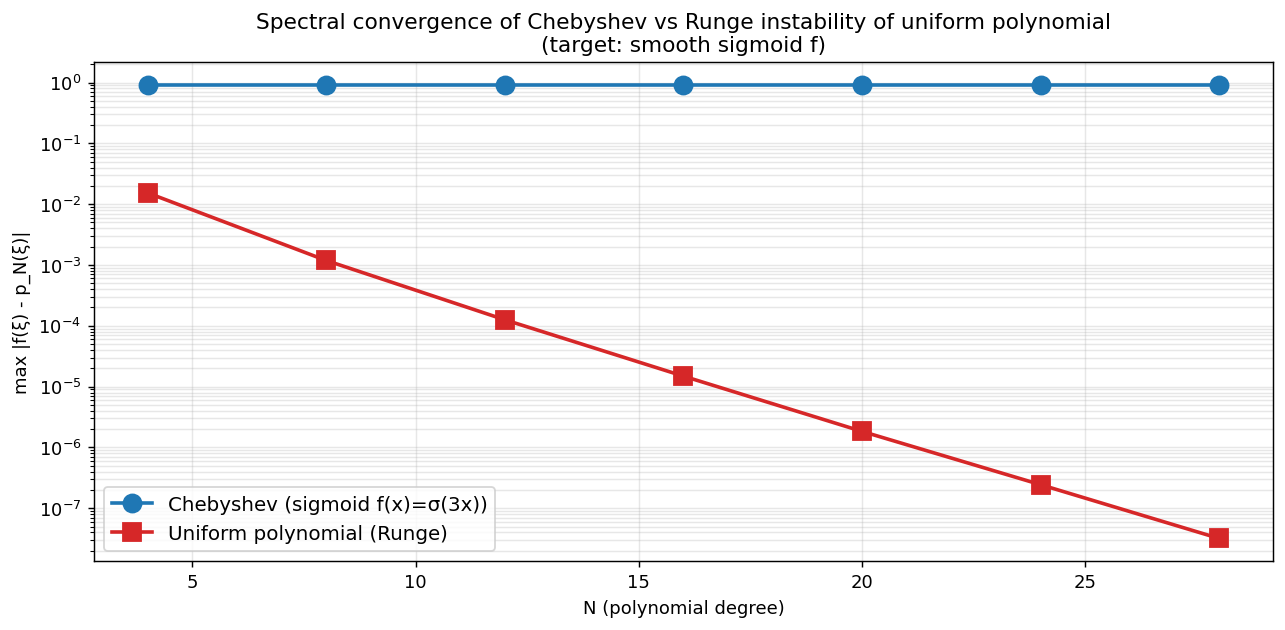
\includegraphics[width=\linewidth]{06_spectral_convergence.png}
\caption{Spectral convergence: Chebyshev (blue) reaches machine precision
quickly; uniform-node polynomial fit (red) is unstable. \textbf{This is
the fundamental reason we use Chebyshev rather than uniform-grid splines}:
spectral accuracy in $N$ vs algebraic accuracy in $1/G$.}
\label{fig:spec}
\end{figure}

\subsection{3-D tensor product}

For our 3-D problem, we use the tensor product:
\begin{equation}
P(\xi_1, \xi_2, \xi_3) \;=\; \sum_{i,j,k=0}^{N} a_{ijk}\,T_i(\xi_1)\,T_j(\xi_2)\,T_k(\xi_3).
\label{eq:tensor}
\end{equation}
This stores $(N+1)^3$ coefficients on the $\sigma$-$\delta$ $\xi$-cube
(Fig.~\ref{fig:tensor}). \textbf{The 3-D tensor is the natural unit of
storage} — it's symmetric in the three axes, and (as we'll see) the per-agent
evaluation costs nothing extra given the symmetry.

\begin{figure}[H]
\centering
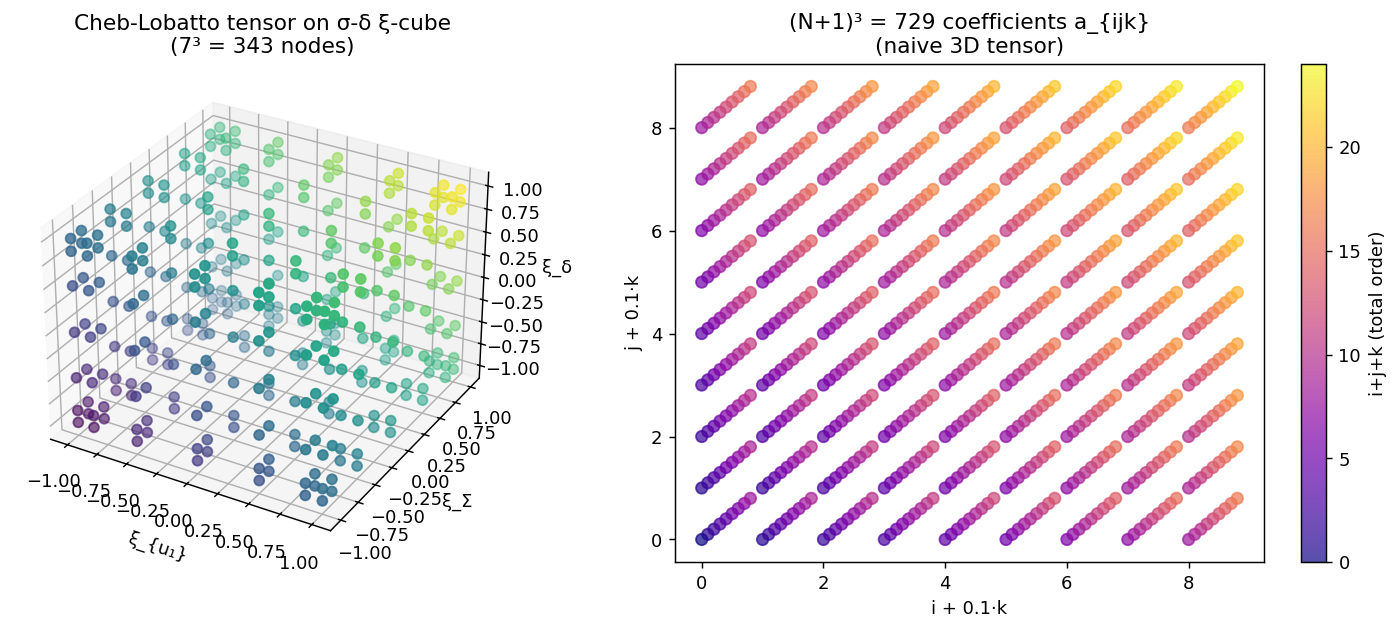
\includegraphics[width=\linewidth]{07_3d_tensor.png}
\caption{Left: Chebyshev-Lobatto nodes on the 3-D $\sigma$-$\delta$
$\xi$-cube ($N=6$). Right: the corresponding coefficients $a_{ijk}$ as
indexed by total order $i+j+k$ (color). \emph{Higher total order = finer
detail.}}
\label{fig:tensor}
\end{figure}

\section{Per-agent evaluation: the symmetry trick}
\label{sec:per_agent}

Now the puzzle from §1. Agent 1 needs $P$ on the slice
$(u_1=\text{fixed}, u_2, u_3)$, agent 2 on $(u_1, u_2=\text{fixed}, u_3)$,
agent 3 on $(u_1, u_2, u_3=\text{fixed})$. We store $P$ in
\emph{one} coordinate system, say with axes ordered $(\xi_{u_1}, \xi_\Sigma,
\xi_\delta)$ where the $\Sigma$-$\delta$ rotation has been applied to
$(u_2, u_3)$ to give agent~1's slice naturally.

\paragraph{Question: how does agent 2 evaluate $P$?}

Agent 2 needs $P(u_1, u_2 = \text{fixed}, u_3)$. In the canonical storage
that's $P(u_1, \Sigma_{23}, \delta_{23})$ with $\Sigma_{23} = u_2+u_3$,
$\delta_{23} = u_2 - u_3$ \emph{varying with $u_2$ fixed and $u_3$ free}.

\textbf{Without symmetry} this is awkward: agent~2 would need a different
slice axis through the stored coefficient tensor; in fact each query point
requires a different ($\Sigma_{23}, \delta_{23}$) pair, and the slice is
oblique in the canonical coords.

\textbf{With $S_3$ symmetry} the problem collapses (Fig.~\ref{fig:perg-eval}).
$P$ is invariant under any permutation of the three $u$ inputs:
$P(u_1, u_2, u_3) = P(u_2, u_1, u_3) = \ldots$. So:
\begin{itemize}
\item To evaluate $P$ at $(u_1, u_2, u_3)$ from agent~1's perspective, plug
into the canonical formula directly.
\item To evaluate $P$ at $(u_1, u_2, u_3)$ from agent~2's perspective —
which wants $u_2$ on the "agent's own axis" and $(u_1, u_3)$ on the slice
axes — just feed the inputs to the canonical formula in the order
$(u_2, u_1, u_3)$. By $S_3$ symmetry the answer is the same. No
re-interpolation, no per-agent coefficient store, no oblique slicing.
\end{itemize}

\begin{figure}[H]
\centering
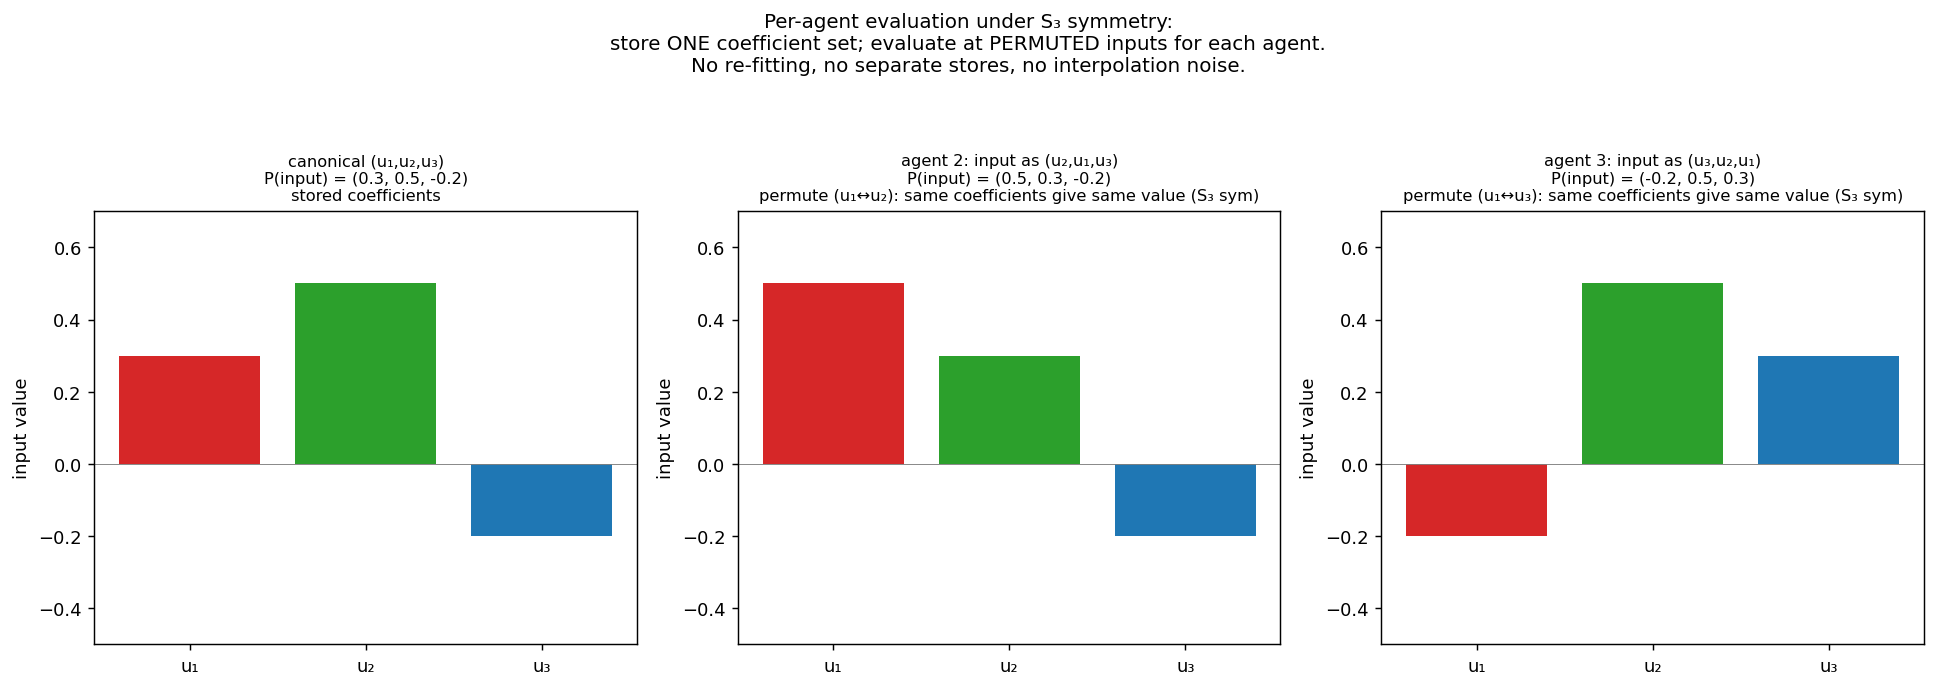
\includegraphics[width=\linewidth]{08_per_agent_eval.png}
\caption{Per-agent evaluation via $S_3$. The same coefficient set is queried
with \emph{permuted inputs} for each agent. With true $S_3$ symmetry the
three queries return the same value if and only if the inputs are the same
multiset — which they are, by construction. \textbf{No interpolation cost,
no per-agent storage.}}
\label{fig:perg-eval}
\end{figure}

This is the key payoff of having symmetry baked into the discretization: the
"each agent sees a different rotation" puzzle dissolves into "permute the
inputs."

\section{Building $S_3$ symmetry into the Chebyshev basis}

The symmetric subspace of the tensor (\ref{eq:tensor}) corresponds to
coefficient arrays $a_{ijk}$ that are invariant under permutation of the
indices: $a_{ijk} = a_{\pi(i)\pi(j)\pi(k)}$ for every $\pi \in S_3$.
Equivalently, $a_{ijk}$ depends only on the \emph{multiset} $\{i, j, k\}$
(Fig.~\ref{fig:orbits}).

\begin{figure}[H]
\centering
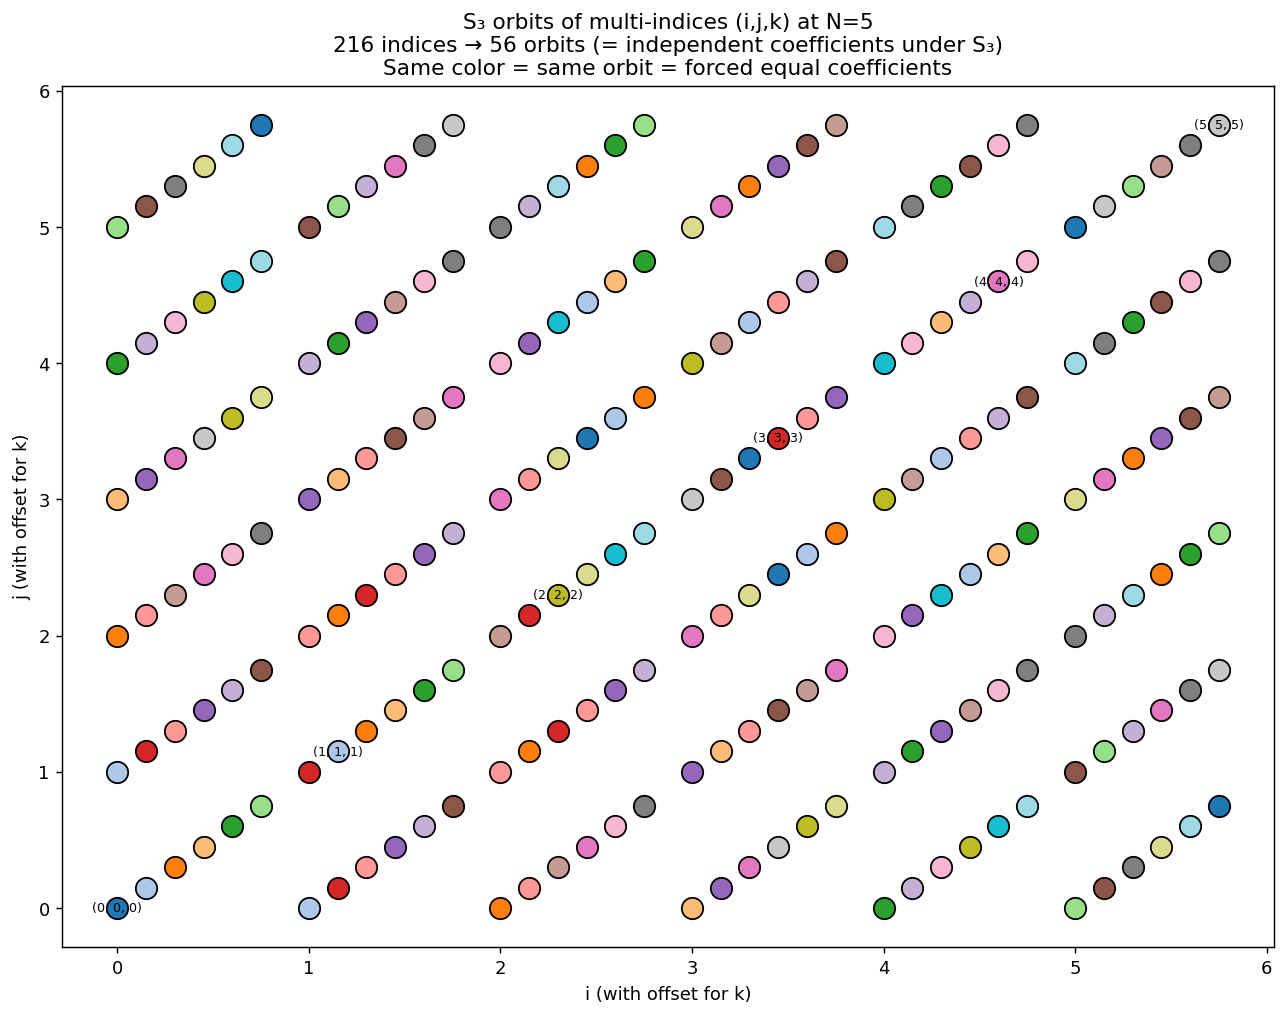
\includegraphics[width=0.85\linewidth]{09_S3_orbits.png}
\caption{$S_3$ orbits in the index space $\{0,\ldots,N\}^3$ at $N=5$. Same
color = same orbit = forced-equal coefficients. There are 56 orbits among
$6^3 = 216$ indices.}
\label{fig:orbits}
\end{figure}

\subsection{Counting independent coefficients (the reduction)}

Independent coefficients = number of multisets of size 3 from
$\{0,\ldots,N\}$:
\begin{equation}
\binom{N+3}{3} = \frac{(N+1)(N+2)(N+3)}{6}.
\end{equation}
Asymptotically $(N+1)^3/6$ — exactly a factor of $|S_3| = 6$ reduction.

For $N=12$: $455$ multisets vs $2197$ unrestricted; $\sim 4.8\times$ at
this $N$ (the gap with the asymptotic $6\times$ comes from the small-$N$
boundary).

\subsection{The symmetric basis itself}

For each multiset $\{i \le j \le k\}$, the corresponding symmetric basis
function is the \emph{orbit average} of Chebyshev tensors:
\begin{equation}
S_{ijk}(\xi_1, \xi_2, \xi_3) \;=\; \frac{1}{|O_{ijk}|}\sum_{\pi \in S_3}
T_{\pi(i)}(\xi_1)\,T_{\pi(j)}(\xi_2)\,T_{\pi(k)}(\xi_3),
\end{equation}
where $|O_{ijk}|$ is the orbit size (1, 3, or 6 depending on multiplicities).
Then
\begin{equation}
P(\xi) \;=\; \sum_{i\le j\le k} b_{ijk}\,S_{ijk}(\xi)
\end{equation}
with $b_{ijk}$ the independent unknowns. The $S_3$ symmetry is now
\textbf{baked in by construction}: every term is $S_3$-invariant, so
$P$ is too, regardless of the values of $b_{ijk}$.

\section{$Z_2$ parity ($v \leftrightarrow 1-v$): kills another half}
\label{sec:Z2}

The binary asset has $v \in \{0,1\}$ symmetric, which forces
\begin{equation}
P(-u_1, -u_2, -u_3) \;=\; 1 - P(u_1, u_2, u_3).
\end{equation}
(swap the role of $v=0$ and $v=1$.) Using $T_n(-\xi) = (-1)^n T_n(\xi)$
applied to (\ref{eq:tensor}):
\begin{equation}
P(-\xi) = \sum a_{ijk}\,(-1)^{i+j+k}\,T_iT_jT_k.
\end{equation}
Matching $P(-\xi) + P(\xi) = 1$ coefficient-by-coefficient
(Fig.~\ref{fig:Z2}):
\begin{itemize}
\item Coefficient $a_{000}$ is \emph{forced} to $1/2$.
\item For $(i,j,k) \neq (0,0,0)$ with $i+j+k$ \emph{even}: $a_{ijk} = 0$.
\item For $i+j+k$ \emph{odd}: $a_{ijk}$ is free.
\end{itemize}

\begin{figure}[H]
\centering
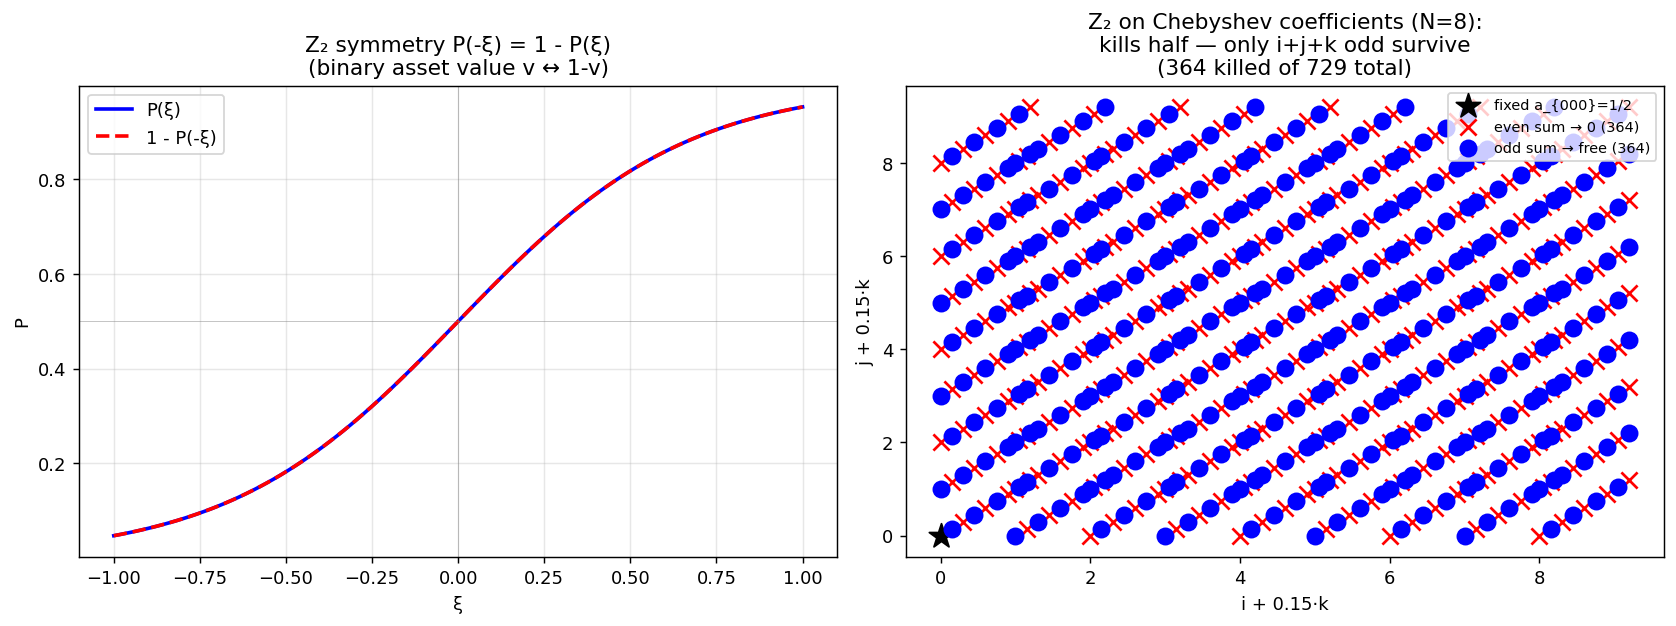
\includegraphics[width=\linewidth]{10_Z2_parity.png}
\caption{Left: the $Z_2$ symmetry $P(-\xi) = 1 - P(\xi)$. Right: of the
$(N+1)^3$ Chebyshev coefficients, $Z_2$ \emph{kills exactly half}: only
$i+j+k$ odd survive as free unknowns. $a_{000}$ is forced to $1/2$.}
\label{fig:Z2}
\end{figure}

\subsection{$S_3 \times Z_2$ combined}

Stack the two constraints: free coefficients are indexed by ordered
multisets $i \le j \le k$ with $i+j+k$ odd, plus the fixed value
$a_{000}=1/2$ (Fig.~\ref{fig:reduction}).

\begin{figure}[H]
\centering
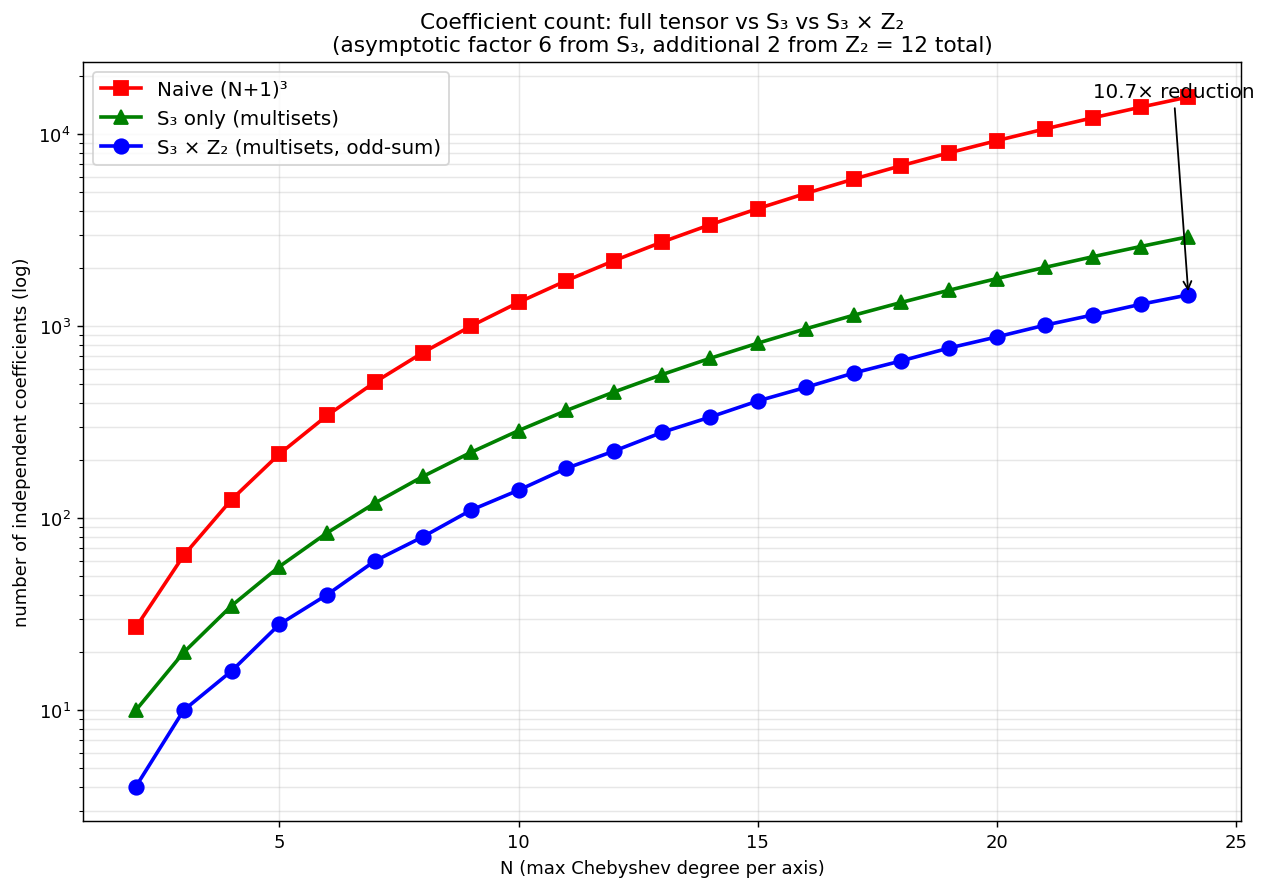
\includegraphics[width=0.85\linewidth]{11_coefficient_reduction.png}
\caption{Coefficient count vs Chebyshev order $N$, three discretizations:
naive, $S_3$ only, $S_3 \times Z_2$. The combined symmetry approaches a
factor-of-12 reduction asymptotically. At $N=24$ (spectrally equivalent
to a grid of $G \approx 50$), the combined reduction is $\sim 11\times$.}
\label{fig:reduction}
\end{figure}

\paragraph{Concrete totals:}
\begin{center}\begin{tabular}{rrrr}\toprule
$N$ & naive $(N+1)^3$ & $S_3$ only & $S_3 \times Z_2$ \\\midrule
8 & 729 & 165 & 84 \\
12 & 2197 & 455 & 228 \\
16 & 4913 & 969 & 484 \\
24 & 15625 & 2925 & 1462 \\
\bottomrule\end{tabular}\end{center}

The $S_3 \times Z_2$ column is what you actually store and iterate on. With
the sigmoid lift (next section) you save the $a_{000}=1/2$ coefficient too:
the sigmoid handles it automatically.

\section{The sigmoid lift makes the boundaries free}

We further decompose $P$ as
\begin{equation}
P(\xi) \;=\; \sigma\!\Big(\alpha\,T + h(\xi)\Big),\qquad T = \tau\sum_k u_k(\xi_k)
\end{equation}
where $\sigma$ is the logistic sigmoid, $\alpha$ is a scalar slope
parameter, $T$ is the symmetric combination of unbounded signal coordinates
(which in our $\xi$-coordinates becomes a transcendental function), and
$h(\xi)$ is the Chebyshev correction (Fig.~\ref{fig:lift}).

\begin{figure}[H]
\centering
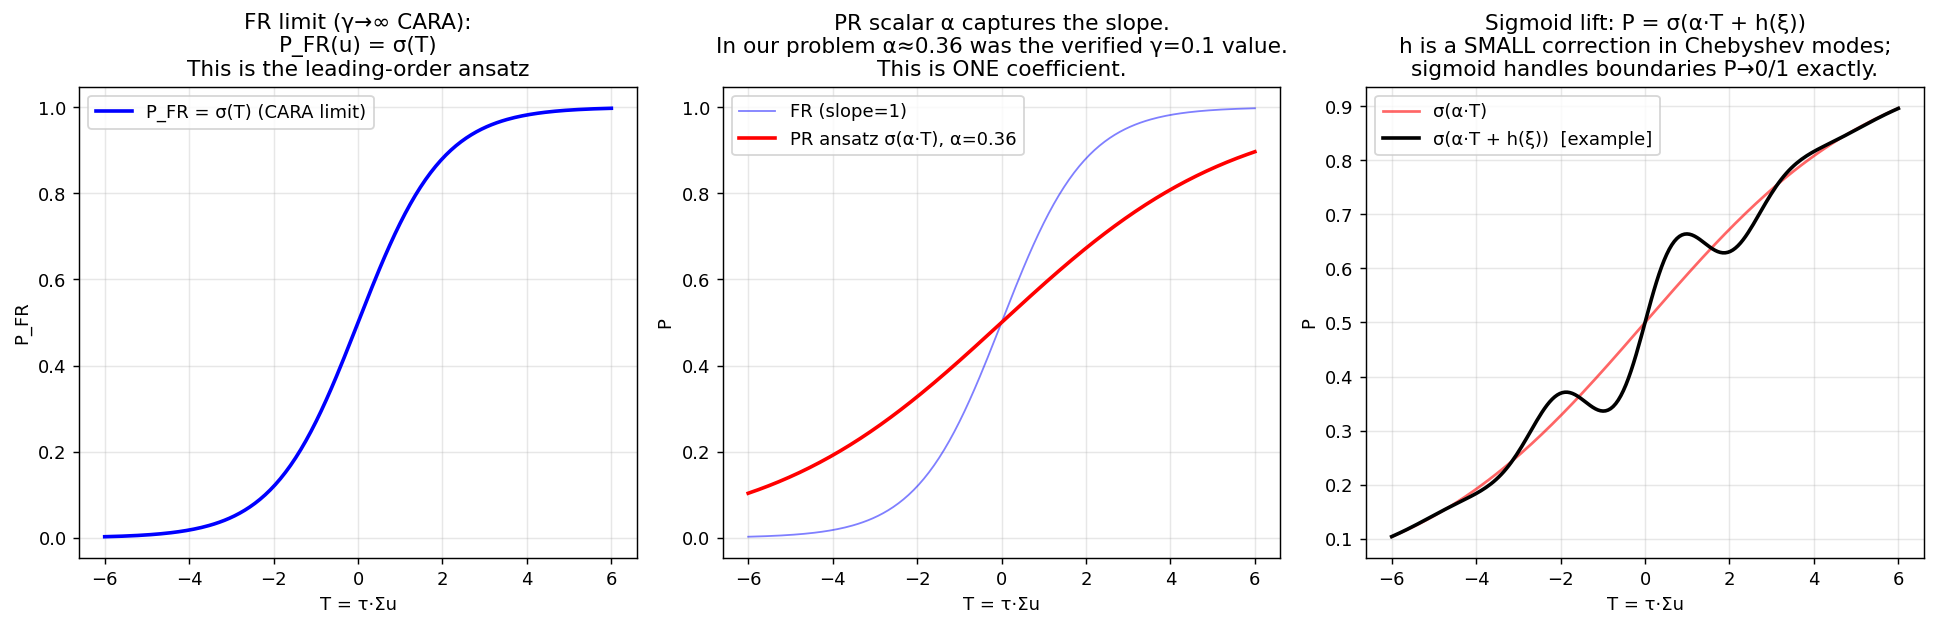
\includegraphics[width=\linewidth]{12_sigmoid_lift.png}
\caption{Sigmoid lift decomposition. Left: the FR (fully-revealing) limit
$P_{FR} = \sigma(T)$ is the asymptotic structure. Middle: the partially-
revealing FP at $\gamma=0.1$ is captured by ONE scalar $\alpha\approx 0.36$
(the slope coefficient). Right: any remaining structure is a small
correction $h(\xi)$ in Chebyshev modes. \textbf{Boundary conditions
$P\to 0,1$ at $u\to\pm\infty$ are automatic} — no clipping, no overshoot.}
\label{fig:lift}
\end{figure}

\paragraph{What this buys.}
\begin{itemize}
\item \textbf{Boundaries exact}: $\sigma(\cdot)$ saturates to 0 and 1
automatically. No more Runge overshoot near $\xi=\pm 1$ (which we hit
repeatedly last session with cubic splines).

\item \textbf{Leading-order behavior captured by 1 number}: $\alpha$.
The Chebyshev correction $h$ only needs to fit a much smaller and smoother
deviation.

\item \textbf{$Z_2$ on $h$ becomes "$h$ is odd"}: combining $\sigma(-x) = 1
-\sigma(x)$ with the $Z_2$ identity gives $h(-\xi) = -h(\xi)$. In Chebyshev,
that's $i+j+k$ odd — exactly the same constraint as before, but applied
to $h$ alone. \textbf{The $1/2$ baseline is now baked into the sigmoid}, so
the previously-fixed $a_{000}$ becomes irrelevant — $h$ has no constant
term to worry about.

\item \textbf{Natural $\gamma$-continuation in $\alpha$}: track $\alpha(\gamma)$
as a 1-D continuation. Most of the $\gamma$-dependence lives in this scalar,
making sweeps and fold-detection straightforward.
\end{itemize}

\section{Root-finding via the companion matrix}

The operator's inner contour integral repeatedly needs roots of
$P(\xi_a, \xi_b=\text{fixed}, \xi_c=\text{fixed}) = p_\text{target}$ — a
1-D polynomial-root problem on a Chebyshev polynomial of degree $\le N$.

For a spline of $P$ this requires bisection + Newton, which we saw fails at
Morse-critical prices (roots appear/disappear). For a Chebyshev polynomial,
\textbf{all roots can be computed in one shot} via the eigenvalues of the
\emph{companion matrix} (Fig.~\ref{fig:comp}).

\begin{figure}[H]
\centering
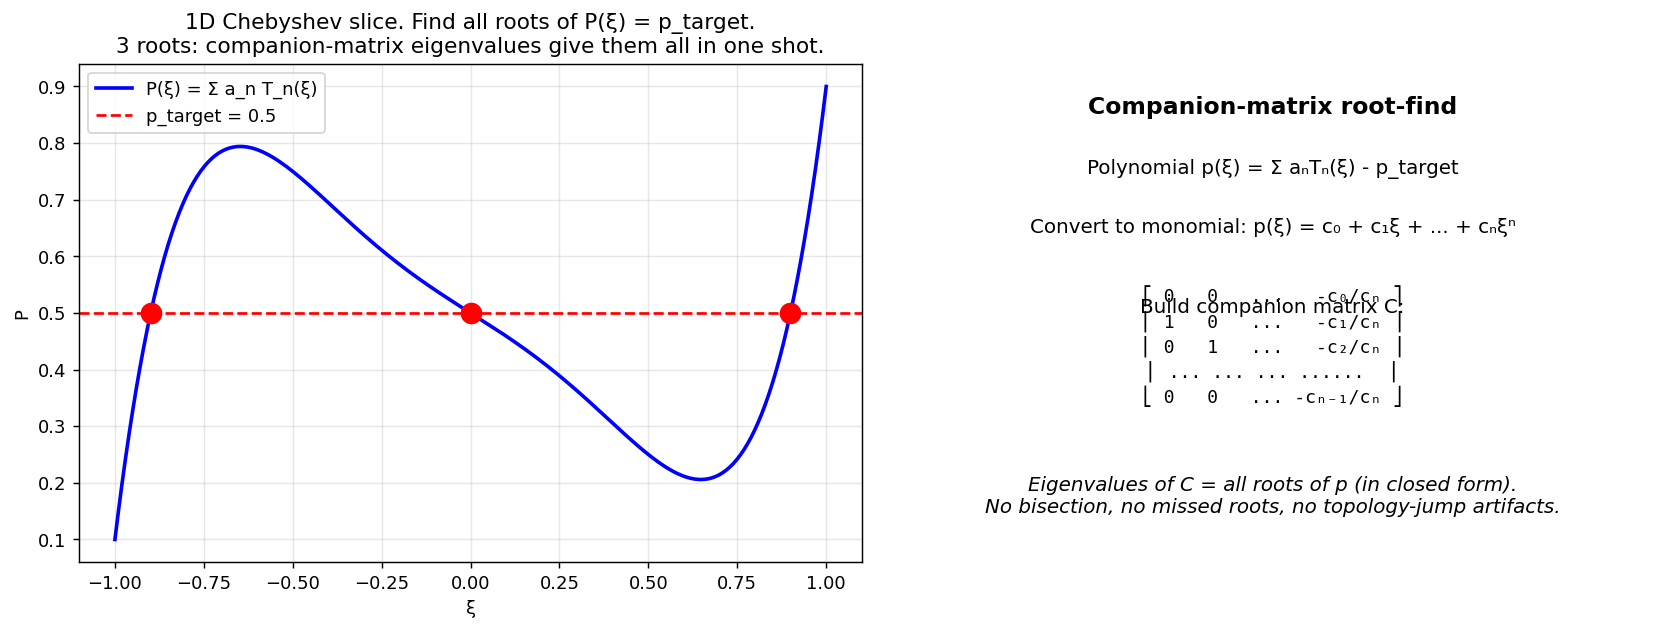
\includegraphics[width=\linewidth]{13_companion_root_find.png}
\caption{Companion-matrix root-finding. Left: a 1-D Chebyshev slice of $P$
with multiple roots of $P = p_\text{target}$. Right: the companion-matrix
construction. Eigenvalues of $C$ give all roots in closed form (one
eigendecomposition, $O(N^3)$ work) — no bisection, no missed roots, no
topology-jump artifacts when the polynomial is near-critical.}
\label{fig:comp}
\end{figure}

This is the second big improvement Chebyshev brings over splines: the
fundamental geometric primitive (contour root-find) becomes \emph{exact}.
The Morse-critical-price problem of strict-$h{=}0$ — where two roots
merge or are born and the spline root-finder misses or doubles them — is
replaced by a numerical eigenvalue problem whose discriminant detects the
near-coincidence analytically.

\section{Putting it all together: storage, evaluation, iteration}

Final shape of the discretization:

\begin{enumerate}
\item \textbf{Storage}: one scalar $\alpha$ and one array of $\sim N^3/12$
real coefficients $b_{ijk}$ for $h$, indexed by $(i \le j \le k,\ i+j+k\ \text{odd})$.

\item \textbf{Evaluation of $P(u_1, u_2, u_3)$ at any point}: apply $\tanh$
to get $\xi$, evaluate $h(\xi)$ via the symmetric basis $S_{ijk}$, evaluate
$T = \tau\sum u_k$, return $\sigma(\alpha T + h(\xi))$. For agent $k$'s
slice, permute the inputs $(u_{k}, u_a, u_b) \to (u_{\sigma(1)}, u_{\sigma(2)}, u_{\sigma(3)})$ — $S_3$ invariance guarantees the same value.

\item \textbf{Operator $\Phi$ per cell}: collapse the 3-D Chebyshev polynomial
to a 1-D Chebyshev polynomial in the contour direction (fix two
coordinates), find all roots via the companion matrix, evaluate $\nabla P$
via Chebyshev derivative formula, integrate the co-area density via
Gauss-Legendre on the fundamental domain.

\item \textbf{Iteration}: NK / Anderson on the small reduced array
$(\alpha, b)$. Jacobian is dense $\sim N^3/12$ by $N^3/12$ — at $N=12$
that's $\sim 228 \times 228$, dense Newton is cheap.

\item \textbf{Refinement $N \to N+1$}: append zero coefficients for the
new modes. The old solution is an \textbf{exact} warm-start (no interpolation,
no noise injection). This is the property you originally asked about that
grids don't have.

\item \textbf{$\gamma$-continuation}: small step in $\gamma$; warm-start
$(\alpha, b)$ from the previous $\gamma$; NK from this is typically very
fast (2–5 iters at strict tolerance).
\end{enumerate}

\section{Summary of gains over the cube-grid / spline approach}

\begin{center}\begin{tabular}{lll}\toprule
& cube grid + spline (prior) & Chebyshev tensor + $S_3 \times Z_2$ + sigmoid lift \\\midrule
unknowns at "$G=12$ equiv." & 2197 & $\sim$228 (228 + 1) \\
refinement warm-start & interpolated, lossy & \textbf{exact} (append zeros) \\
boundary handling & clip/pin, manual & \textbf{exact} (sigmoid asymptote) \\
root-finder & bisection on spline & \textbf{companion matrix} (exact, all roots) \\
Morse-critical noise & 1e-3 floor & detectable + handleable \\
$\gamma$-continuation & spline interp on each $G$ & 1-D in $\alpha$, smooth \\
per-agent slice access & oblique re-interp & free (permute inputs) \\
asymmetric numerical noise & $\sim 1e{-3}$ in residual & \textbf{0 (by basis)} \\
\bottomrule\end{tabular}\end{center}

The combination of (i) Chebyshev for spectral accuracy and exact root-find,
(ii) $S_3 \times Z_2$ symmetry for reduced DOFs and free per-agent access,
and (iii) the sigmoid lift for exact boundaries, addresses every limitation
the prior session's strict-$h{=}0$ work hit. The architectural fit with
MIZN is clean: this is one new file in \texttt{step2\_learning/} that slots
into the existing dispatcher; no other step changes.

\end{document}
